Tuy nhiên, sử dụng RAG đơn giản
thì độ chính xác chưa cao
và vẫn có thể sai sót
vì vậy,
em sử dụng LangGraph
xây dựng Agentic RAG
để tăng độ chính xác
và hạn chế ảo giác
vì miền tư vấn pháp luật
yêu cầu độ chính xác cao.
% \end{block}
Thay vì thực thi các bước theo quy trình tuyến tính như LangChain, LangGraph mô hình hóa luồng công việc dưới dạng một đồ thị gồm các thành phần chính sau:

\begin{itemize}

\item Nodes (Nút): Đại diện cho các bước xử lý, tác vụ hoặc hành động cụ thể, chẳng hạn như gọi mô hình ngôn ngữ lớn (LLM), truy xuất CSDL hoặc tương tác với người dùng.
\item Edges (Cạnh): Xác định hướng chuyển tiếp giữa các nút. Các cạnh có thể là đường đi trực tiếp hoặc cạnh có điều kiện (conditional edges), cho phép lựa chọn nhánh thực thi dựa trên kết quả của nút trước đó.
\item Cycles (Vòng lặp): Đây là đặc điểm nổi bật của LangGraph. Khác với kiến trúc đồ thị có hướng không chu trình, LangGraph cho phép tác nhân (agent) quay lại các nút đã thực hiện để đánh giá lại kết quả, tự sửa lỗi hoặc lặp lại quy trình nhiều lần cho đến khi đạt được mục tiêu mong muốn.
\item State (Trạng thái): Đây là bộ nhớ dùng chung. Mọi nút (node) trong đồ thị đều có thể đọc dữ liệu từ State này và ghi kết quả mới của chúng vào đây.
\end{itemize}

\begin{figure}[H]
\centering
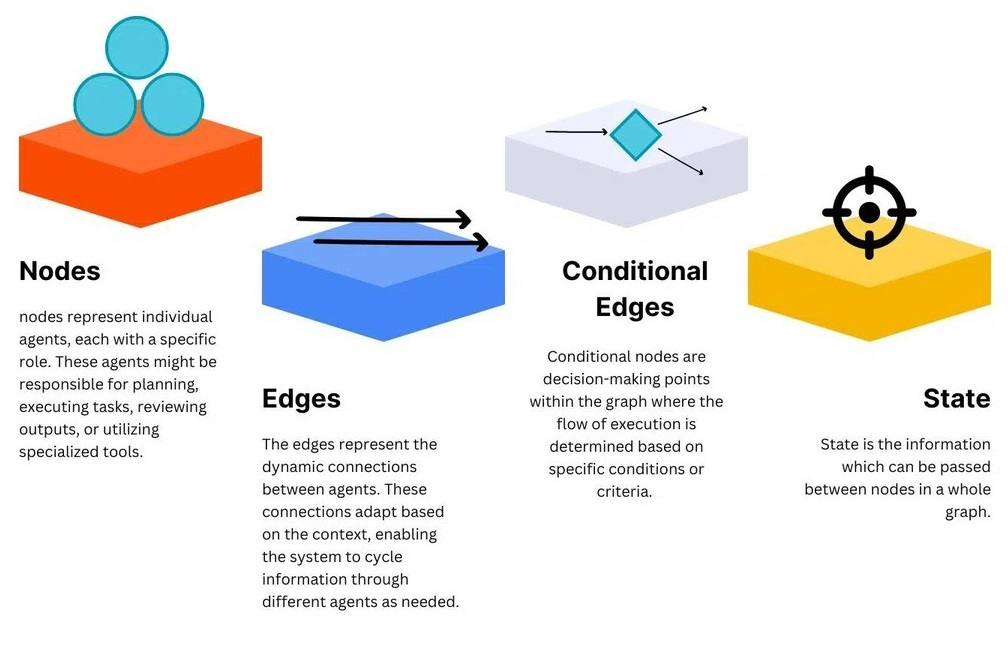
\includegraphics[scale = 0.5]{pictures/625723062_18126048418556935_1835132745978934341_n.jpg}
\caption{Các khái niệm quan trọng của LangGraph}
\end{figure}

Sơ đồ Agentic RAG dự án này:

\begin{figure}[H]
\centering
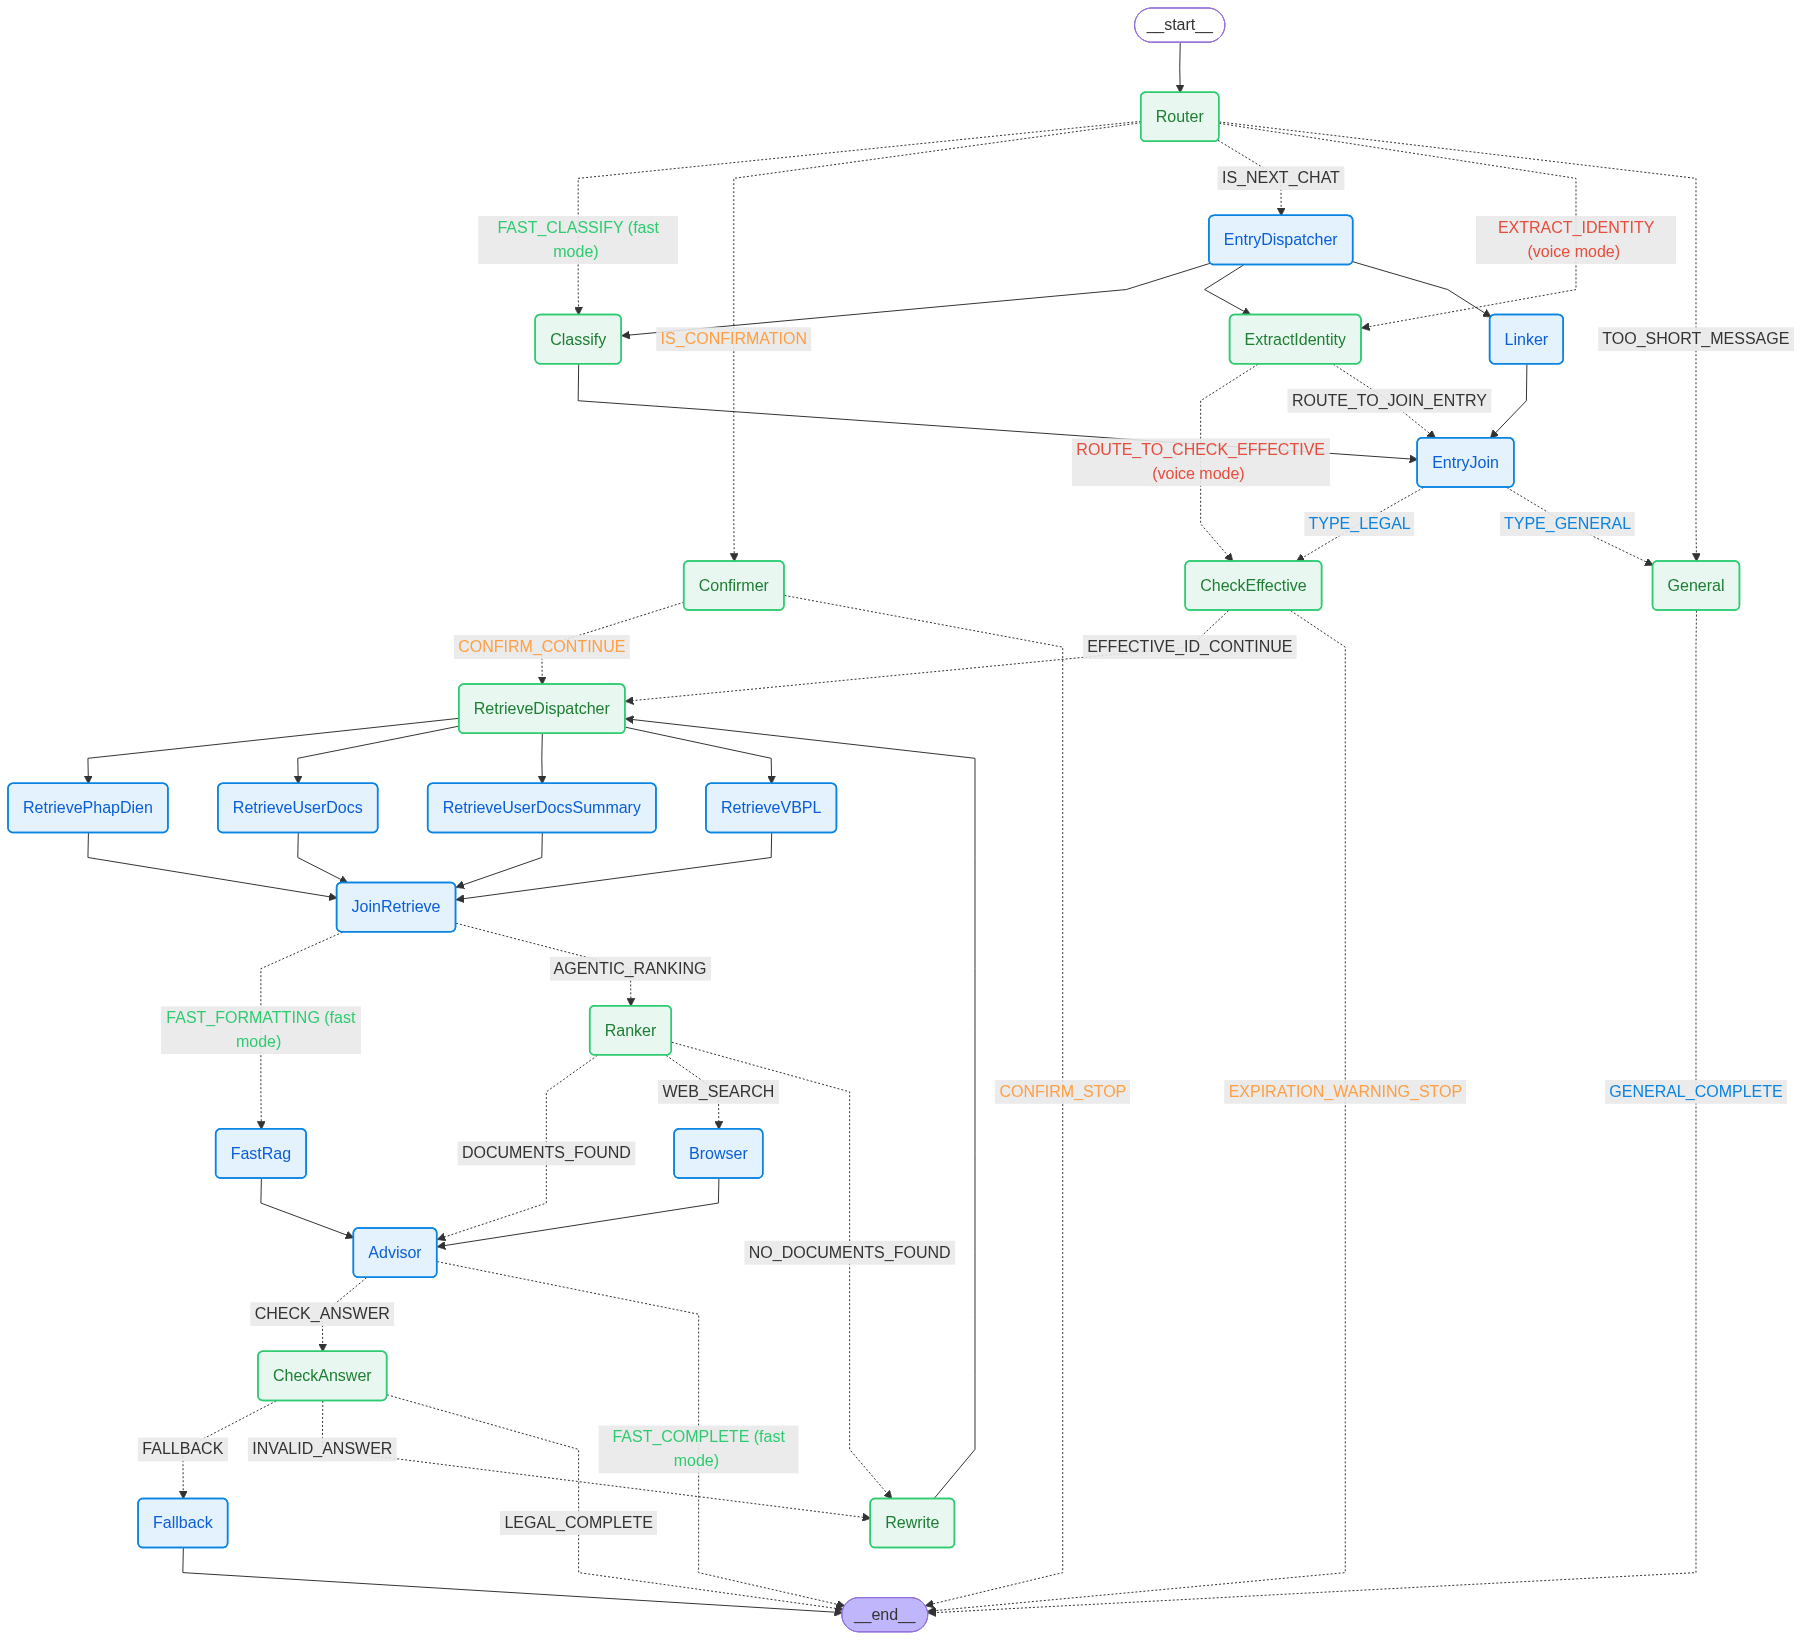
\includegraphics[scale = 0.23]{pictures/rag_diagram.png}
\caption{Sơ đồ LangGraph của dự án}
\end{figure}

Giải thích sơ đồ Agentic RAG:

\begin{itemize}
\item Hệ thống
phân chia việc sử dụng thông minh
giữa mô hình nhỏ cho luồng cơ bản
và mô hình lớn cho tác vụ suy luận
là chìa khóa để tối ưu cả chi phí, độ trễ và hiệu năng.
(Nhìn vào sơ đồ các Node màu xanh lá sử dụng mô hình nhỏ,
các Node màu xanh dương sử dụng mô hình lớn)

\item Mỗi tin nhắn đều đi qua \texttt{Router}.
Node này kiểm tra điều kiện
giúp định tuyến vào luồng chính xác
theo từng trạng thái.

\item Ở chế độ suy luận Agentic RAG đầy đủ
thực hiện
phân tích song song

\begin{itemize}

\item \texttt{Linker} đọc URL nếu có.
\item \texttt{Classify} phân loại câu hỏi là pháp lý hay thông thường.
\item \texttt{Extract Identity} trích xuất số hiệu văn bản (VD: \texttt{100/2019/NĐ-CP}).

\end{itemize}

\item Kiểm tra hiệu lực pháp lý:
Nếu câu hỏi thuộc nhóm \texttt{TYPE\_LEGAL} và có số hiệu văn bản,
hệ thống tra cứu trạng thái.

\begin{itemize}

\item Văn bản đã hết hiệu lực hoàn toàn
thì kết thúc ngay.
\item Văn bản hết hiệu lực một phần
thì phát cảnh báo và chờ người dùng xác nhận ở lượt sau qua \texttt{Confirmer}.

\end{itemize}

\item Truy xuất nguồn dữ liệu song song

\begin{itemize}

\item Tài liệu người dùng (Milvus)
\item Tóm tắt tài liệu (Cloudflare R2)
\item Văn bản pháp luật (Pinecone)
\item Dữ liệu pháp điển (Qdrant)

\end{itemize}

\item Tiếp tục tới \texttt{Ranker} để lọc tài liệu

\begin{itemize}

\item Nếu có tài liệu hợp lý
thì
chuyển đến \texttt{Advisor}
để tiến hành tạo câu trả lời.

\item Nếu không có tài liệu hợp lý
thì
chuyển đến \texttt{Rewrite}
để tạo lại câu hỏi.

\item Sau khi thử tạo lại câu hỏi
vẫn không có tài liệu hợp lý
thì sẽ dùng \texttt{Browser}
để lấy tài liệu
tại nguồn
thuvienphapluat.vn và luatvietnam.vn

\end{itemize}

\item Vòng lặp tự kiểm tra chất lượng
Sau khi \texttt{Advisor} trả lời,
\texttt{Check Answer} đánh giá câu trả lời có hợp lý hay không?

\begin{itemize}

\item Nếu không hợp lệ và chưa quá 2 lần
thì xóa câu trả lời cũ,
chuyển đến \texttt{Rewrite}
để tạo lại câu hỏi
và
lặp lại toàn bộ luồng truy xuất.

\item Nếu câu trả lời hợp lệ hoặc đã quá số lần thử lại
thì
hệ thống kết thúc quá trình trả lời.
\end{itemize}

\item Ở chế độ Fast RAG
chỉ đi qua \texttt{Classify} để phân loại.
Sau đó truy xuất dữ liệu lấy dữ liệu.
Dùng \texttt{Advisor} trả lời
và
hệ thống kết thúc quá trình trả lời
mà không cần bước kiểm tra.

\item Ở chế độ giọng nói Voice,
do đã có Agent nên không cần qua bước phân loại của LangGraph
và người dùng không thể nhập URL nên hệ thống chuyển đến \texttt{Extract Identity} trích xuất số hiệu văn bản.

\end{itemize}
